\documentclass{beamer}

\usepackage{amsmath}
\usepackage{graphics}
\usepackage{framed}
\usepackage{amssymb}

\begin{document}
\begin{frame}
\textbf{\texttt{R} for Economic and Social Research}
\begin{enumerate}
\item \texttt{R} Packages and Taskviews, 10 packages
\item Official Statistics and Survey 
\item Regular Expressions with \texttt{R}
\item Econometric Tools: AER and Forecase
\item The HadleyVerse : ggplot and dplyr
\item Other Matters:  Julia and GitHub
\item Instructional Design : DataCamp
\end{enumerate}

\end{frame}
%=================================================================== %
\begin{frame}
% % SLIDE 1 - COVER SLIDE
\begin{figure}
\centering

\includegraphics[width=0.7\linewidth]{Rlogo}
\end{figure}
\LARGE
\[ \mbox{Using R for Economic and Social Research} \]	



\end{frame}



%=================================================================== %
\begin{frame}[fragile]
	
	
	\begin{figure}
\centering
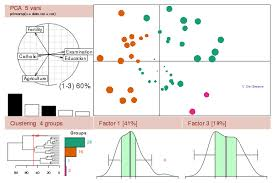
\includegraphics[width=0.7\linewidth]{CRAN}
\caption{Comprehensive R Archive Network}

\end{figure}
	
	
\end{frame}



%=================================================================== %
\begin{frame}[fragile]
	
\frametitle{Packages}
\begin{itemize}
\item The CRAN package repository features 6107 available packages. 
\item Packages contain
various functions and data sets for numerous purposes, e.g.
\textbf{\textit{ggplot2}} package, \textbf{\textit{AER}} package, \textbf{\textit{survival}} package, etc.
\item Some packages are part of the basic installation. Others can be
downloaded from CRAN.
\item To access all of the functions and data sets in a particular package,
it must be loaded into the workspace. 
\item For example, to load the
\textbf{\textit{ggplot2}} package:
\end{itemize}
\begin{framed}
\begin{verbatim}
install.packages(ggplot2)
library(ggplot2)
\end{verbatim}
\end{framed}
\end{frame}
%=================================================================== %
\begin{frame}	
\frametitle{R Packages}

\begin{itemize}
\item ``10 R packages I wish I knew about earlier" - Drew Conway (Yhat.com, February 2013)
\bigskip \item ``The HadleyVerse" - Hadley Wickham
\begin{itemize}
	
	\item  ggplot2, dplyr, reshape, lubridate, stringr
	
	\item  With Romain Francois, Dianne Cook and Garret Grolemund.
\end{itemize}
\bigskip
\item Dr Brendan Haplin (UL): lme4 ,TraMineR, Gelman's arm, MASS, foreign. 
\bigskip
\item Shiny - Web Applications with \texttt{R}
\end{itemize}
\end{frame}



%=================================================================== %
\begin{frame}
\frametitle{The forecast Package}	
	
forecast makes it incredibly easy to fit time series models like ARIMA, ARMA, AR, Exponential Smoothing, etc.

	
	
\end{frame}


%=================================================================== %
\begin{frame}
	\frametitle{The forecast Package}	
	
	\begin{figure}
\centering
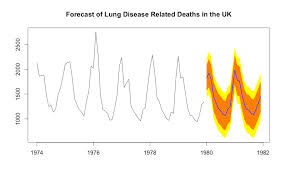
\includegraphics[width=0.7\linewidth]{forecast}

\end{figure}

	
	
\end{frame}
%=================================================================== %
\begin{frame}
	
	
	
	
	\begin{figure}
\centering
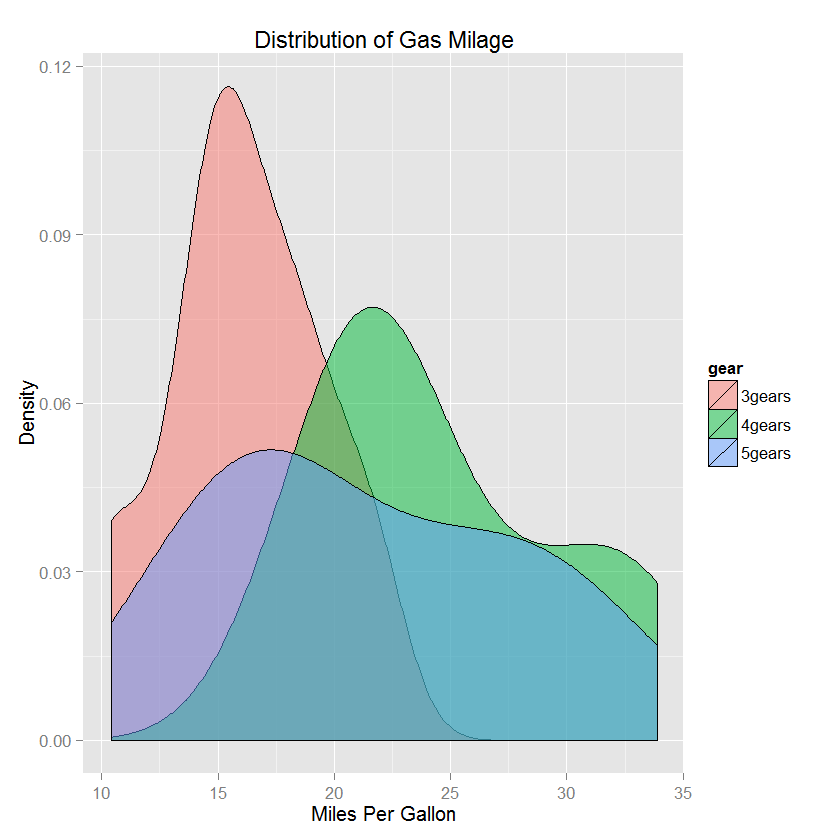
\includegraphics[width=0.9\linewidth]{ggplotdensity}
\caption{}
\label{fig:ggplotdensity}
\end{figure}

\end{frame}





%=================================================================== %
\begin{frame}
	
	
	
	
	\begin{figure}
\centering
\includegraphics[width=0.45\linewidth]{"ASDAbook cover"}
\caption{Springer's UseR! series}
\end{figure}

\end{frame}
%=================================================================== %
\begin{frame}[fragile]
\Large
\begin{framed}
\begin{verbatim}
"As usual, NZ is ahead of the pack and 
@statisticsnz is the first govt 
statistics agency to deploy 
rstudio server pro! #rstats"

                      Hadley Wickham, 
                      (11th December).
\end{verbatim}
\end{framed}

\end{frame}
%=================================================================== %
\begin{frame}	
	
\frametitle{Tidy Data}
\textbf{\textit{Revision}}\\
What are the three characteristics of tidy data?

\begin{itemize}
	\item ``\textit{\textbf{Tidy data}}" by Hadley Wickham (RStudio)
	\item Submission to Journal of Statistical Software
	\item (http://vita.had.co.nz/papers/tidy-data.pdf)
\end{itemize}

\end{frame}
%============================================================================ %
%ESRItalk
\begin{frame}

Three Principles from Hadley Wickham's paper
\begin{itemize}
	\item[1.] Each variable forms a column, 
	\item[2.] Each observation forms a row, 
	\item[3.] Each table/file stores data about one kind of observation.
\end{itemize}
\end{frame}
%============================================================================ %



\begin{frame}
\frametitle{dplyr : Grammar of data manipulation}
	\begin{itemize}
\item dplyr is a new package which provides a set of tools for efficiently manipulating datasets in R.
\item dplyr is the next iteration of plyr, focussing on only data frames. \item dplyr is faster, has a more consistent API and should be easier to use. 
	\end{itemize}


\end{frame}
%============================================================= %
\begin{frame}
\frametitle{dplyr : Grammar of data manipulation}
(abstract by Hadley Wickahm)

There are three key ideas that underlie dplyr:

1) Your time is important, so Romain Francois has written the key pieces in Rcpp to provide blazing fast performance. Performance will only get better over time, especially once we figure out the best way to make the most of multiple processors. 

\end{frame}
%============================================================= %
\begin{frame}
2) Tabular data is tabular data regardless of where it lives, so you should use the same functions to work with it. 

With dplyr, anything you can do to a local data frame you can also do to a remote database table. PostgreSQL, MySQL, SQLite and Google bigquery support is built-in; adding a new backend is a matter of implementing a handful of S3 methods. 
\end{frame}
%============================================================= %
\begin{frame}
\frametitle{dplyr : Grammar of data manipulation}
3) The bottleneck in most data analyses is the time it takes for you to figure out what to do with your data, and dplyr makes this easier by having individual functions that correspond to the most common operations  group\_by, summarise,mutate, filter, select and arrange). Each function does one only thing, but does it well.

\end{frame}	
	
%ESRItalk
\begin{frame}[fragile]
The American Community Survey distributes downloadable data about United States communities. 
Download the 2006 microdata survey about housing for the state of Idaho using \texttt{download.file()} from here: 

\begin{verbatim}
https://dl.dropbox.com/u/7710864/data/csv_hid/ss06hid.csv

or here:

https://spark-public.s3.amazonaws.com/dataanalysis/ss06hid.csv 
\end{verbatim}
and load the data into \texttt{R}. 
\end{frame}
%=========================================================================== %

% You will use this data for the next several questions. 
\begin{frame}[fragile]
\noindent \textbf{\textit{Code Book}}\\
The code book, describing the variable names is here: 

\begin{verbatim}
https://dl.dropbox.com/u/7710864/data/PUMSDataDict06.pdf

or here: 

https://spark-public.s3.amazonaws.com/dataanalysis/PUMSDataDict06.pdf
\end{verbatim}
\end{frame}
%=========================================================================== %
\begin{frame}[fragile]

How many housing units in this survey were worth more than \$1,000,000?
% **53**

%\begin{framed}
%	\begin{verbatim}
%	# Download 2006 microdata survey 
%	# re: housing for Idaho using download.file()
%	# setwd("~/DA")
%	download.file(
%	'https://spark-public.s3.amazonaws.com/dataanalysis/ss06hid.csv',
%	"ss06hid.csv", method="curl")
%	
%	# Download the code book:
%	# download.file(
%	'https://spark-public.s3.amazonaws.com/dataanalysis/PUMSDataDict06.pdf',
%	"PUMSDataDict06.pdf", method="curl")
%	\end{verbatim}
%\end{framed}

\end{frame}

%=========================================================================================== %

\begin{frame}[fragile]

\begin{framed}
	\begin{verbatim}	
	# load the data into R
	idahoData <- read.csv("ss06hid.csv", header=TRUE)
	
	# Is it just Idaho data?
	table(idahoData$ST)
	#Check the PDF - what does 16 mean?
	
	#any missing data?
	summary(idahoData$ST)
	
	# How many housing units are worth
	# more than $1,000,000?
	table(idahoData$TYPE,idahoData$VAL)
	\end{verbatim}
\end{framed}

\end{frame}

%=========================================================================================== %

\begin{frame}[fragile]

\begin{framed}
	\begin{verbatim}
	#from local files
	idahoData <- read.csv("daquiz2.csv", header=TRUE)
	
	\end{verbatim}
\end{framed}

\end{frame}

%=========================================================================================== %

\begin{frame}[fragile]
\frametitle{Question 4}

\begin{itemize}
	\item Use the data you loaded from Question 3. 
	\item Consider the variable FES. 
	\item Which of the "tidy data" principles does this variable violate?
\end{itemize}

%%READY
%\textbf{\textit{Revision}}\\
%What are the three characteristics of tidy data?
%
%\begin{itemize}
%	\item ``\textit{\textbf{Tidy data}}" by Hadley Wickham (RStudio)
%	\item Submission to Journal of Statistical Software
%	\item (http://vita.had.co.nz/papers/tidy-data.pdf)
%\end{itemize}
%Three Principles from Hadley Wickham's paper
%\begin{itemize}
%	\item[1.] Each variable forms a column, 
%	\item[2.] Each observation forms a row, 
%	\item[3.] Each table/file stores data about one kind of observation.
%\end{itemize}

\begin{framed} 
	\begin{verbatim}
	# let's look!
	unique(idahoData$FES)
	\end{verbatim}
\end{framed} 

\end{frame}
%-----------------------------------------------------------------%

%\subsection*{ Question 5 }
\begin{frame}


\textbf{Options}
\begin{itemize}
	\item[(i)]  Each tidy data table contains information about only one type of observation.\\
	(Not so)
	
	\item[(ii)]  Each variable in a tidy data set has been transformed to be interpretable.
	(No)
	
	\item[(iii)]  Tidy data has no missing values.
	
	\item[(iv)]  Tidy data has one variable per column.
\end{itemize}
\end{frame}
%-----------------------------------------------------------------%

%\subsection*{ Question 5 }
\begin{frame}[fragile]
Use the data you loaded from Question 3. 

\begin{itemize}
	\item How many households have 3 bedrooms and and 4 total rooms? 
	\item How many households have 2 bedrooms and 5 total rooms? 
	\item How many households have 2 bedrooms and 7 total rooms?
\end{itemize}
\begin{framed}
	\begin{verbatim}
	#USING TABLE
	#Rooms on Rows , Bedrooms on Columns
	#dnn adds dimension names
	
	table(idahoData$RMS,idahoData$BDS,dnn=list("RMS","BDS"))
	
	\end{verbatim}
\end{framed}

\end{frame}
%============================================================= %
\begin{frame}[fragile]
Another Way of Doing it
\begin{framed}
	\begin{verbatim}
	# How many households have 3 bedrooms and 4 total rooms?
	nrow(idahoData[!is.na(idahoData$BDS) & idahoData$BDS==3 &
	!is.na(idahoData$BDS) & idahoData$RMS==4,])
	# How many households have 2 bedrooms and 5 total rooms?
	nrow(idahoData[!is.na(idahoData$BDS) & idahoData$BDS==2 &
	!is.na(idahoData$BDS) & idahoData$RMS==5,])
	# How many households have 2 bedrooms and 7 total rooms?
	nrow(idahoData[!is.na(idahoData$BDS) & idahoData$BDS==2 &
	!is.na(idahoData$BDS) & idahoData$RMS==7,])
	
	\end{verbatim}
\end{framed}
% **148, 386, 49**
\end{frame}

%-----------------------------------------------------------------%

%\subsection*{Question 6}
\begin{frame}
\begin{itemize}
	\item Use the data from Question 3. 
	\item Create a logical vector that identifies the households on greater than 10 acres who sold more than \$10,000 worth of agriculture products. 
	\item Assign that logical vector to the variable `\texttt{agricultureLogical}`. 
	\item Apply the `\texttt{which()} function like this to identify the rows of the data frame where the logical vector is `TRUE`.
\end{itemize}

\end{frame}
%====================================================== %
\begin{frame}[fragile]
\begin{framed} 
	\begin{verbatim}
	# Like this (this wont run yet)
	which(agricultureLogical) 
	\end{verbatim}
\end{framed} 
\end{frame}
%====================================================== %
\begin{frame}[fragile]
What are the first 3 values that result?

\begin{framed} \begin{verbatim}
	# Showing off a bit
	q6cols <- c("ACR", "AGS")
	which(names(idahoData) %in% q6cols)  
	
	# logical vector
	agricultureLogical <- idahoData$ACR==3 & idahoData$AGS==6
	
	# and:
	which(agricultureLogical) 
	\end{verbatim}\end{framed} 

%**125, 238, 262**
\end{frame}
%====================================================== %
\begin{frame}
	
\frametitle{Question 7}

\begin{itemize}
	\item Use the data from Question 3. 
	\item Create a logical vector that identifies the households on greater than 10 acres who
	sold more than \$10,000 worth of agriculture products. 
	\item Assign that logical vector to the variable \texttt{agricultureLogical}. 
	\item Apply the \texttt{which()} function like this to identify the rows of the 
	data frame where the logical vector is TRUE and assign it to the variable indexes. 
\end{itemize}

\end{frame}
%====================================================== %
\begin{frame}[fragile]
	
\begin{framed} 
\begin{verbatim}
	indexes =  which(agricultureLogical) 
\end{verbatim}
\end{framed} 

If your data frame for the complete data is called \texttt{dataFrame} you can create a data frame 
with only the above subset with the command: 

\end{frame}
%====================================================== %
\begin{frame}[fragile]
	
\begin{framed} 
	\begin{verbatim}
	subsetDataFrame  = dataFrame[indexes,] 
	\end{verbatim}
\end{framed} 

\noindent Note that we are subsetting this way because the NA values in the variables 
will cause problems if you subset directly with the logical statement. 

\end{frame}
%====================================================== %
\begin{frame}[fragile]
	
\noindent How many households in the subsetDataFrame have a missing value for the mortgage status 
(MRGX) variable?

\begin{framed} 
	\begin{verbatim}
	indexes <- which(agricultureLogical)
	subsetIdahoData <- idahoData[indexes,]
	
	# And then:
	nrow(subsetIdahoData[is.na(subsetIdahoData$MRGX),])
	\end{verbatim}
\end{framed} 

\end{frame}
%====================================================== %
\begin{frame}[fragile]
	
\frametitle{Question 8}
\begin{itemize}
	\item Use the data from Question 3.
	\item Apply `\texttt{strsplit()}` to split all the names of the data frame on the characters "wgtp". 
	\item What is the value of the 123 element of the resulting list?
\end{itemize}

\begin{framed} \begin{verbatim}
	List <- strsplit(names(idahoData), "wgtp")
	List[123]
	\end{verbatim}\end{framed} 

%**"" "15"**
\end{frame}
%====================================================== %
\begin{frame}[fragile]
\frametitle{Question 9}

What are the 0\% and 100\% quantiles of the variable \texttt{YBL}? Is there anything wrong with these values?
\textit{ Hint: you may need to use the \texttt{na.rm} parameter.}

\begin{framed} 
	\begin{verbatim}
	quantile(idahoData$YBL, na.rm=TRUE)
	#  0%  25%  50%  75% 100% 
	#  -1    3    5    7   25 
	\end{verbatim}
\end{framed} 

\end{frame}
%====================================================== %
\begin{frame}[fragile]	
\frametitle{Question 10}

In addition to the data from Question 3, the American Community Survey also collects data about populations. 
Using `\texttt{download.file()}`, download the population record data from: 

\begin{verbatim}
https://dl.dropbox.com/u/7710864/data/csv_hid/ss06pid.csv 

or here:

https://spark-public.s3.amazonaws.com/dataanalysis/ss06pid.csv
\end{verbatim}

\end{frame}
%====================================================== %
\begin{frame}[fragile]
	
\begin{itemize}
	\item Load the data into \texttt{R}. Assign the housing data from Question 3 to a data frame `\texttt{housingData}` and the population data from above to a data frame `populationData`.
	
	\item Use the merge command to merge these data sets based only on the common identifier "SERIALNO". 
	
	\item What is the dimension of the resulting data set? 
\end{itemize}
%[OPTIONAL] For fun, you might look at the data and see what happened when they merged.

\end{frame}
%========================================================================================== %
\begin{frame}[fragile]
	
%	download.file(
%	'https://spark-public.s3.amazonaws.com/dataanalysis/ss06pid.csv',
%	'ss06pid.csv', method='curl')
%	
\textbf{Merging Data Sets}
\begin{framed} 
	\begin{verbatim}

	housingData <- read.csv("ss06hid.csv", header=TRUE)
	popuData <- read.csv("ss06pid.csv", header=TRUE)
	
	dim(merge(housingData, 
	popuData, by="SERIALNO", all=TRUE))
	\end{verbatim}
\end{framed} 

\end{frame}
% **number of rows = 15451, number of columns = 426**

\end{document}
